% Options for packages loaded elsewhere
\PassOptionsToPackage{unicode}{hyperref}
\PassOptionsToPackage{hyphens}{url}
%
\documentclass[
]{book}
\usepackage{amsmath,amssymb}
\usepackage{iftex}
\ifPDFTeX
  \usepackage[T1]{fontenc}
  \usepackage[utf8]{inputenc}
  \usepackage{textcomp} % provide euro and other symbols
\else % if luatex or xetex
  \usepackage{unicode-math} % this also loads fontspec
  \defaultfontfeatures{Scale=MatchLowercase}
  \defaultfontfeatures[\rmfamily]{Ligatures=TeX,Scale=1}
\fi
\usepackage{lmodern}
\ifPDFTeX\else
  % xetex/luatex font selection
\fi
% Use upquote if available, for straight quotes in verbatim environments
\IfFileExists{upquote.sty}{\usepackage{upquote}}{}
\IfFileExists{microtype.sty}{% use microtype if available
  \usepackage[]{microtype}
  \UseMicrotypeSet[protrusion]{basicmath} % disable protrusion for tt fonts
}{}
\makeatletter
\@ifundefined{KOMAClassName}{% if non-KOMA class
  \IfFileExists{parskip.sty}{%
    \usepackage{parskip}
  }{% else
    \setlength{\parindent}{0pt}
    \setlength{\parskip}{6pt plus 2pt minus 1pt}}
}{% if KOMA class
  \KOMAoptions{parskip=half}}
\makeatother
\usepackage{xcolor}
\usepackage{longtable,booktabs,array}
\usepackage{calc} % for calculating minipage widths
% Correct order of tables after \paragraph or \subparagraph
\usepackage{etoolbox}
\makeatletter
\patchcmd\longtable{\par}{\if@noskipsec\mbox{}\fi\par}{}{}
\makeatother
% Allow footnotes in longtable head/foot
\IfFileExists{footnotehyper.sty}{\usepackage{footnotehyper}}{\usepackage{footnote}}
\makesavenoteenv{longtable}
\usepackage{graphicx}
\makeatletter
\def\maxwidth{\ifdim\Gin@nat@width>\linewidth\linewidth\else\Gin@nat@width\fi}
\def\maxheight{\ifdim\Gin@nat@height>\textheight\textheight\else\Gin@nat@height\fi}
\makeatother
% Scale images if necessary, so that they will not overflow the page
% margins by default, and it is still possible to overwrite the defaults
% using explicit options in \includegraphics[width, height, ...]{}
\setkeys{Gin}{width=\maxwidth,height=\maxheight,keepaspectratio}
% Set default figure placement to htbp
\makeatletter
\def\fps@figure{htbp}
\makeatother
\setlength{\emergencystretch}{3em} % prevent overfull lines
\providecommand{\tightlist}{%
  \setlength{\itemsep}{0pt}\setlength{\parskip}{0pt}}
\setcounter{secnumdepth}{5}
% definitions for citeproc citations
\NewDocumentCommand\citeproctext{}{}
\NewDocumentCommand\citeproc{mm}{%
  \begingroup\def\citeproctext{#2}\cite{#1}\endgroup}
\makeatletter
 % allow citations to break across lines
 \let\@cite@ofmt\@firstofone
 % avoid brackets around text for \cite:
 \def\@biblabel#1{}
 \def\@cite#1#2{{#1\if@tempswa , #2\fi}}
\makeatother
\newlength{\cslhangindent}
\setlength{\cslhangindent}{1.5em}
\newlength{\csllabelwidth}
\setlength{\csllabelwidth}{3em}
\newenvironment{CSLReferences}[2] % #1 hanging-indent, #2 entry-spacing
 {\begin{list}{}{%
  \setlength{\itemindent}{0pt}
  \setlength{\leftmargin}{0pt}
  \setlength{\parsep}{0pt}
  % turn on hanging indent if param 1 is 1
  \ifodd #1
   \setlength{\leftmargin}{\cslhangindent}
   \setlength{\itemindent}{-1\cslhangindent}
  \fi
  % set entry spacing
  \setlength{\itemsep}{#2\baselineskip}}}
 {\end{list}}
\usepackage{calc}
\newcommand{\CSLBlock}[1]{\hfill\break\parbox[t]{\linewidth}{\strut\ignorespaces#1\strut}}
\newcommand{\CSLLeftMargin}[1]{\parbox[t]{\csllabelwidth}{\strut#1\strut}}
\newcommand{\CSLRightInline}[1]{\parbox[t]{\linewidth - \csllabelwidth}{\strut#1\strut}}
\newcommand{\CSLIndent}[1]{\hspace{\cslhangindent}#1}
% Ensure text is aligned to the left margin
\usepackage{geometry}
\geometry{
  left=1in,    % Adjust these margins as necessary
  right=1in,
  top=1in,
  bottom=1in,
  bindingoffset=0in
}

% Disable paragraph indentation
\setlength{\parindent}{0pt}
\ifLuaTeX
  \usepackage{selnolig}  % disable illegal ligatures
\fi
\usepackage{bookmark}
\IfFileExists{xurl.sty}{\usepackage{xurl}}{} % add URL line breaks if available
\urlstyle{same}
\hypersetup{
  pdftitle={Course Notes - Introduction to Analytics Modeling},
  pdfauthor={Nolan MacDonald},
  hidelinks,
  pdfcreator={LaTeX via pandoc}}

\title{Course Notes - Introduction to Analytics Modeling}
\author{Nolan MacDonald}
\date{Fall 2024}

\begin{document}
\maketitle

{
\setcounter{tocdepth}{1}
\tableofcontents
}
\chapter{Module 1 - Introduction}\label{module-1---introduction}

\section{M1L1 - Course Overview}\label{m1l1---course-overview}

\section{M1L2 - Course Structure}\label{m1l2---course-structure}

\section{M1L2a - Homework Grading and Q\&A}\label{m1l2a---homework-grading-and-qa}

\subsection{Homework Format}\label{homework-format}

The main focus of the homework will be your analysis of your results, \textbf{not your code.}
For a top score, you shouldn't just run some code and display some results; rather, you should also discuss the results qualitatively, point out anything surprising, and comment on possible explanations.
The top recommended forms for your analysis, in order, are: pdf, html, txt, and then word doc.

We recommend \textbf{not} including your name / e-mail in your homework PDF.
We (TAs) and the system will know who you are, and submitting anonymously will not cause any problems assigning your grade later.
It will also avoid potential problems of bias.

\subsection{Grading Homeworks}\label{grading-homeworks}

Once you've submitted your homework, you will have to complete 3-Peer Reviews.
You are given a rubric with \textbf{scoring guidelines with possible values of 100, 90, 75, 50, and 0.}
When doing the grading, Canvas does allow you to give options outside of the scale, but please stick to it.
I can see who gave the off-scale score, and it only frustrates your fellow students and makes my job a little harder.
Also, if you have a homework marked as ``late'' in your grading queue, please grade it as normal.
We have a very small tolerance between when peer reviews are assigned and homeworks are due to allow for students who had technical issues to submit.

\begin{itemize}
\tightlist
\item
  100 is ``All correct (perhaps except a few details) with a deeper solution than expected''

  \begin{itemize}
  \tightlist
  \item
    This means that if students gave answers that delved deeper into the analytical methods and modeling techniques with appropriate solutions and explanations etc, then that constitutes a 100. All questions are completed. \textbf{When giving this grade, please comment what you believe the person did well and how they went above and beyond.} I cannot force you to leave a comment, but it will help stay consistent with the regrading policy that will be mentioned later.
  \end{itemize}
\item
  90 is for ``most or all correct.''

  \begin{itemize}
  \tightlist
  \item
    This means that student provided code, answered the questions asked with code output, and provided reasonable but basic explanations for their answers. There can be minor errors like slight inconsistencies or minor misunderstandings. All questions are answered. \textbf{This is the ``default'' grade. If a student does what is asked, and provides reasonable explanation for their work, but doesn't go above and beyond, this is their grade.} While comments here can be nice, if you have nothing else to add other than ``they did everything right,'' you do not have to leave a comment.
  \end{itemize}
\item
  75 is ``not correct, but a reasonable attempt.''

  \begin{itemize}
  \tightlist
  \item
    There is some code, solutions, and explanation, but the explanation is faulty, incorrect, or non-existent or the solution values are completely different than outlined in the homework solutions or solutions and explanation do not make sense. At least half of the questions are answered/attempted including the coding questions. \textbf{When giving this grade, please comment what you believe the person did that was fundamentally incorrect.} This will help the student learn and will also help me in case of a regrade request.
  \end{itemize}
\item
  50 is ``Not correct, insufficient effort.''

  \begin{itemize}
  \tightlist
  \item
    There is a distinct lack of effort on homework like no code, no answers, no explanations, or little of any of these. Particularly, if a student only answers a descriptive problem (one which involves answering a prompt) and does none of the coding problems, then this would also be considered insufficient effort. \textbf{When giving this grade, please comment what you believe the person did that was fundamentally incorrect and explain what part of the homework they did not do.} This will help the student learn and will also help me in case of a regrade request.
  \end{itemize}
\item
  0 is ``Not Submitted''

  \begin{itemize}
  \tightlist
  \item
    There is nothing of merit submitted. The student did not attempt the problems, just submitted random or unrelated work to try and obtain a 50. \textbf{When giving this grade, it is because the student literally had nothing there, was completely unrelated (a picture of a ham-sandwich), or basically un-attempted.} If you feel like the student was just being lazy, you most likely should give them a zero.
  \end{itemize}
\item
  Other info: Optional truly means optional. Doing an optional part does not guarantee a 100. On the other end, You can still get a 100 even if you don't do an optional part. An optional part can contribute to a deeper analysis, but isn't required nor does it guarantee it.
\item
  Please try to be helpful with your comments if you provide any.

  \begin{itemize}
  \tightlist
  \item
    Also, try to provide appropriate feedback or comments based on the homework questions being asked.
  \item
    For example, I could say that ``exploring more C values for Q2.2.1 would have shown a wider range/change in the~model accuracy'' or ``using different kernels would result in higher model accuracy''

    \begin{itemize}
    \tightlist
    \item
      These comments are appropriate but do not result in a drop in the student's grade since exploring different kernels was optional and we did not give a specific range of C values to look at.
    \end{itemize}
  \end{itemize}
\end{itemize}

\section{M1L3 - Modeling}\label{m1l3---modeling}

\chapter{Module 2 - Classification}\label{module-2---classification}

\section{M2L1 - Introduction to Classification}\label{m2l1---introduction-to-classification}

\section{M2L2 - Choosing a Classifier}\label{m2l2---choosing-a-classifier}

\section{M2L3 - Data Definitions}\label{m2l3---data-definitions}

\section{M2L4 - Support Vector Machines (SVMs)}\label{m2l4---support-vector-machines-svms}

\section{M2L5 - SVM: What the Name Means}\label{m2l5---svm-what-the-name-means}

\section{M2L6 - Advanced Support Vector Machines}\label{m2l6---advanced-support-vector-machines}

\section{M2L7 - Scaling and Standardization}\label{m2l7---scaling-and-standardization}

\section{M2L8 - K-Nearest-Neighbor (KNN) Algorithm}\label{m2l8---k-nearest-neighbor-knn-algorithm}

\chapter{Module 3 - Validation}\label{module-3---validation}

\section{Overview}\label{overview}

Module 3 will continue with basic machine learning algorithms.
The modules will cover couple of cross-cutting concepts and the important topic of model validation.

Additional References:

\citeproc{ref-arlot2010survey}{{[}1{]}}. \href{https://www.di.ens.fr/willow/pdfs/2010_Arlot_Celisse_SS.pdf}{A Survey of Cross-Validation Procedures for Model Selection}

\section{M3L1 - Introduction to Validation}\label{m3l1---introduction-to-validation}

Validation

\begin{itemize}
\tightlist
\item
  How good is the model?
\end{itemize}

Data has two types of patterns

\begin{itemize}
\tightlist
\item
  \textbf{Real Effect} - Real relationship between attributes and response
\item
  \textbf{Random Effect} - Random, but looks like a real effect
\end{itemize}

Fitting matches both real and random effects

\begin{itemize}
\tightlist
\item
  Real effects - Same in all data sets
\item
  Random effects - Different in all data sets
\end{itemize}

\textbf{Example: What day of the month were you born?}

\begin{itemize}
\tightlist
\item
  Training Data: 3, 21, 24, 24, 25, 26, 27, 30, 30, 31
\item
  Best Predictor: You were born on the 26th

  \begin{itemize}
  \tightlist
  \item
    Right in the middle of 9/10 data points
  \end{itemize}
\item
  \textbf{This is a random effect!}
\item
  This model using 9/10 from 21-31 doesn't have a large error
\item
  If new data showed 2, 9, 11, 12, 14, 21, 24, 24, 29, 31

  \begin{itemize}
  \tightlist
  \item
    Much larger error due to the uniform spread over the month
  \end{itemize}
\item
  Was this just luck? (3, 21, 24, etc.)

  \begin{itemize}
  \tightlist
  \item
    No, some random pattern would have shown up

    \begin{itemize}
    \tightlist
    \item
      Early in month
    \item
      Middle of month
    \item
      Even/odd numbered day
    \item
      Day is multiple of 3
    \item
      Day is close to one of my kids birthdays
    \item
      Etc.
    \end{itemize}
  \end{itemize}
\end{itemize}

\subsection{M3L1 - Summary}\label{m3l1---summary}

\begin{itemize}
\tightlist
\item
  The example proves we can't measure the model's effectiveness on data it was trained on
\item
  Model fit captures real and random effects
\item
  Only real effects are duplicated in other data
\end{itemize}

\emph{Don't judge a model based on how well it fits the training data}.

\begin{itemize}
\tightlist
\item
  Validation is crucial to determine how good a model is and how accurately it performs on new data
\item
  Measuring a model's performance on the same training data used to create it is not a good approach, as it will be too optimistic
\item
  Any dataset contains both real effects (true relationships) and random effects (patterns that occur by chance)
\item
  When fitting a model to training data, it captures both real and random effects
\item
  However, when using the model on new data, only the real effects will persist, while the random effects will be different
\item
  An example is given of a silly model that predicts people's birth dates based on a random pattern in the training data, which would not generalize well
\item
  The key takeaway is that we cannot rely on training data performance to evaluate a model - we need a separate validation process to get an accurate assessment of its effectiveness
\end{itemize}

\section{M3L2 - Validation and Test Data Sets}\label{m3l2---validation-and-test-data-sets}

\textbf{Measure a model's performance:}

\begin{itemize}
\tightlist
\item
  A larger set of data to fit the model
\item
  A smaller set of data to measure the model's effectiveness
\end{itemize}

Splitting Data:

\begin{itemize}
\tightlist
\item
  Training set (larger) to fit model
\item
  Validation set (smaller) to estimate effectiveness
\end{itemize}

Training and Validation Sets:

\begin{itemize}
\tightlist
\item
  Observed performance = real quality + random effects

  \begin{itemize}
  \tightlist
  \item
    High-performing models more likely to have \emph{above-average random effects}
  \end{itemize}
\item
  Observed performance of chosen model is \emph{probably too optimistic}
\end{itemize}

Test Sets:

\begin{itemize}
\tightlist
\item
  Training data set to fit the models
\item
  Validation data set to choose best model
\item
  Test data set to estimate performance of chosen model
\end{itemize}

Overall:

\begin{itemize}
\tightlist
\item
  Training Set - Building models
\item
  Validation Set - Picking a model
\item
  Test Set - Estimating performance of chosen model
\end{itemize}

\subsection{Summary}\label{summary}

\begin{itemize}
\tightlist
\item
  Using only training data to evaluate a model's performance is often too optimistic, as the model overfits to random patterns in the training data.
\item
  \textbf{To get a better measure of performance, we use separate validation and test sets:}

  \begin{itemize}
  \tightlist
  \item
    Training set: Used to fit/build the model
  \item
    Validation set: Used to evaluate and compare different models
  \item
    Test set: Used to get an unbiased final estimate of the chosen model's performance
  \end{itemize}
\item
  The validation set helps select the best model, but its performance estimate may still be inflated due to random chance when choosing the ``best'' model.
\item
  The test set provides a final unbiased performance estimate for the selected model.
\item
  \textbf{General process:}

  \begin{itemize}
  \tightlist
  \item
    Train multiple models on training data
  \item
    Evaluate models on validation set and select best one
  \item
    Estimate final performance of chosen model on test set
  \end{itemize}
\item
  This three-way split helps avoid overfitting and provides a more realistic assessment of how well the model will generalize to new data.
\item
  There are different ways to split data into training, validation and test sets, which will be covered in a future lesson.
\end{itemize}

\textbf{The key takeaway is that using separate datasets for training, model selection, and final evaluation helps produce more reliable and generalizable machine learning models.}

\section{M3L3 - Splitting Data}\label{m3l3---splitting-data}

\begin{itemize}
\tightlist
\item
  Training data too optimistic so we need to use a test set
\item
  Training data set to build model
\item
  Validation set to compare models
\item
  Test set to estimate performance of chosen model
\end{itemize}

\textbf{How do we split data into traning, validation, and test sets?}

\begin{itemize}
\tightlist
\item
  Method 1: Random - Randomly choose data points
\item
  Method 2: Rotation - Take turns selecting points
\end{itemize}

\textbf{Training-Validation-Training-Test-Training}

\begin{itemize}
\tightlist
\item
  Randomness could give one set more early or late data

  \begin{itemize}
  \tightlist
  \item
    Rotation equally separates data
  \end{itemize}
\item
  Rotation may introduce bias
\end{itemize}

\subsection{Summary}\label{summary-1}

\begin{itemize}
\tightlist
\item
  Data needs to be split into training, validation, and test sets to properly evaluate model performance.
\item
  \textbf{Recommended splits:}

  \begin{itemize}
  \tightlist
  \item
    For two sets: 70-90\% training, 10-30\% testing (Rule of thumb)
  \item
    For three sets:

    \begin{itemize}
    \tightlist
    \item
      50\% training, 25\% validation, 25\% testing
    \item
      60\% training, 20\% validation, 20\% testing
    \item
      70\% training, 15\% validation, 15\% testing
    \end{itemize}
  \end{itemize}
\item
  \textbf{Two main approaches for splitting data:}

  \begin{itemize}
  \tightlist
  \item
    Simple randomness: Randomly assign data points to each set
  \item
    Rotation: Systematically rotate through assigning points to each set
  \end{itemize}
\item
  \textbf{Advantages of rotation:}

  \begin{itemize}
  \tightlist
  \item
    Ensures equal representation of data across time periods
  \item
    Avoids potential biases from random sampling
  \end{itemize}
\item
  \textbf{Disadvantages of rotation:}

  \begin{itemize}
  \tightlist
  \item
    May introduce other biases if not done carefully (e.g.~only certain days of week in each set)
  \end{itemize}
\item
  A hybrid approach combining randomness and rotation can be used to avoid biases.
\item
  Cross-validation is another technique for using data, which will be covered in a future lesson.
\end{itemize}

\textbf{It is important to properly split data to get accurate model evaluations, while there are tradeoffs between different splitting approaches.}

\section{M3L4 - Cross-Validations}\label{m3l4---cross-validations}

\begin{itemize}
\item
  What if important data only appears in validation or test sets? \emph{Use cross-validation!}
\item
  Use of \texttt{k} in analytics

  \begin{itemize}
  \tightlist
  \item
    k-means
  \item
    k-nearest neighbor
  \item
    k-fold cross validation
  \end{itemize}
\end{itemize}

\textbf{k-fold Cross-Validation}

\begin{itemize}
\tightlist
\item
  For each of the \texttt{k} parts:

  \begin{itemize}
  \tightlist
  \item
    Train the model on all the other parts
  \item
    Evaluate it on the one remaining part
  \end{itemize}
\item
  \emph{Average the k evaluations to estimate the model's quality}
\item
  No standard number for \texttt{k}, but \texttt{k=10} is common
\end{itemize}

\begin{figure}

{\centering 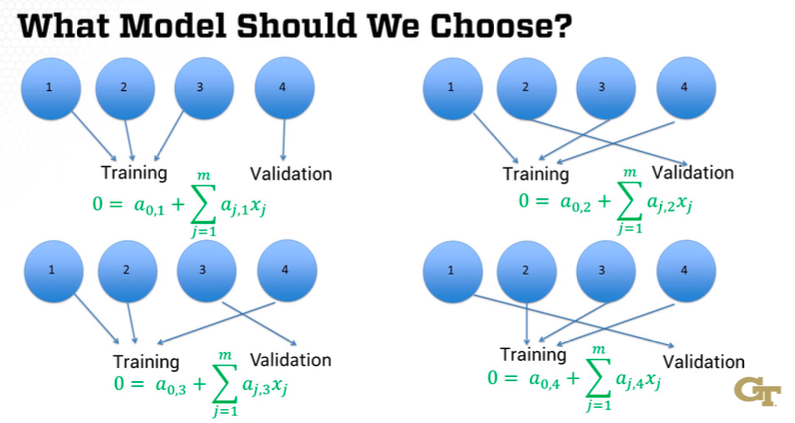
\includegraphics[width=1\linewidth]{figures/m3-l4-k-fold} 

}

\caption{k-Fold Cross Validation}\label{fig:unnamed-chunk-1}
\end{figure}

\textbf{ANSWER: NONE!}

\begin{itemize}
\tightlist
\item
  Do not average the coefficients over four splits
\item
  Train the model again using all the data
\end{itemize}

k-Fold Cross-Validation provides:

\begin{itemize}
\tightlist
\item
  Better use of data
\item
  Better estimate of model quality
\item
  Choose model more effectively
\end{itemize}

\subsection{Summary}\label{summary-2}

\begin{itemize}
\tightlist
\item
  \textbf{Purpose of Cross-Validation:} Cross-validation is introduced as a technique to ensure that important data points are not excluded from the training set, which can happen if they only appear in the validation or test sets. This method helps in making better use of the data available.
\item
  \textbf{Types of Cross-Validation:} The lecture specifically discusses k-fold cross-validation, a popular method in analytics. The `k' in k-fold cross-validation indicates the number of parts the data is split into for training and validation purposes.
\item
  \textbf{Process of K-Fold Cross-Validation:}

  \begin{itemize}
  \tightlist
  \item
    The data is divided into k parts. For example, if k=4, the data is split into four parts.
  \item
    The model is trained on k-1 parts and validated on the remaining part. This process is repeated k times, with each part being used as the validation set once.
  \item
    Every data point is used for training in k-1 models, ensuring no important data is left out.
  \end{itemize}
\item
  \textbf{Model Evaluation:} The performance of the model is evaluated by averaging the results from the k different validation sets. This average provides an estimate of the model's quality.
\item
  \textbf{Choosing the Final Model:} After using cross-validation to select a model, the final model is retrained using all the data parts together. This ensures the model benefits from the full dataset.
\item
  \textbf{Common Practice:} While there is no standard number for k, using k=10 is common in practice.
\end{itemize}

\textbf{Overall, cross-validation is emphasized as a crucial step in model selection and evaluation, helping to improve the reliability of the analytics process.}

\chapter{Module 4 - Clustering}\label{module-4---clustering}

\section{Overview}\label{overview-1}

Module 4 will continue with basic machine learning algorithms.
The focus will be on clustering models.
The modules will cover couple of cross-cutting concepts, including distance norms, and k-means clustering.

Additional References:

\citeproc{ref-wikibookskmeans}{{[}2{]}}. \href{https://en.wikibooks.org/wiki/Data_Mining_Algorithms_In_R/Clustering/K-Means}{Data Mining Algorithms In R/Clustering/K-Means}

\section{M4L1 - Introduction to Clustering}\label{m4l1---introduction-to-clustering}

\textbf{Clustering:} An unsupervised machine learning technique designed to group unlabeled examples based on their similarity to each other.

\begin{itemize}
\tightlist
\item
  Grouping data points
\item
  \emph{Important to note: If the examples are labeled, the grouping is called classification}
\end{itemize}

Examples of Clustering:

\begin{itemize}
\tightlist
\item
  Targeted marketing/market segmentation

  \begin{itemize}
  \tightlist
  \item
    Potential customers need a message that would be most likely to encourage them to buy
  \end{itemize}
\item
  For example, if we were selling a SUV:

  \begin{itemize}
  \tightlist
  \item
    Size
  \item
    Price
  \item
    Versatility
  \item
    Coolness
  \end{itemize}
\item
  Each set of people would be a cluster
\item
  We would try to use data to split consumers into sets to discover what marketing they should be shown
\item
  You can examine a cluster and it may not always be correct, which can help you find a meaningful cluster in your data

  \begin{itemize}
  \tightlist
  \item
    For example, we did not consider gas mileage
  \end{itemize}
\item
  Other examples:

  \begin{itemize}
  \tightlist
  \item
    Targeted marketing/market segmentation
  \item
    Personalized medicine
  \item
    Locating facilities - Look at where people live and provide a police station for each cluster
  \item
    Image analysis - CAPCHA
  \item
    Initial data investigation
  \end{itemize}
\end{itemize}

\section{M4L2 - Distance Norms}\label{m4l2---distance-norms}

The choice of distance measures is important in clustering.
Distance measures define how the similarity of the two element are calculated and influences the shape of the clusters.

\textbf{Euclidean (straight-line) distance:}

\begin{itemize}
\tightlist
\item
  Distance in Euclidean space by length of straight line segment between two points
  \[
  distance = \sqrt{\sum^n_{i=1}(x_i - y_i)^2} = \sqrt{(x_1-y_1)^2+(x_2-y_2)^2}
  \]
\end{itemize}

\textbf{Rectilinear (Manhattan) Distance:}

\begin{itemize}
\tightlist
\item
  Commonly used in city planning with a grid, hence Manhattan term
  \[
  distance = \sum^n_{i=1} |x_i-y_i| =  |x_1-y_1| + |x_2-y_2|
  \]
\end{itemize}

\textbf{Minkowski (p-norm) Distance:}

\begin{itemize}
\tightlist
\item
  We can describe both euclidean (p=2) and rectilinear (p=1) distance with p-norm (or Minkowski) distance
  \[
  distance = \sqrt[p]{\sum^n_{i=1} |x_i-y_i|^p} = \sqrt[p]{|x_1-y_1|^p + |x_2-y_2|^p}
  \]
\end{itemize}

The most common values for p include 1, 2, and \(\infty\) (\(\infty\)-norm distance).

\textbf{Infinity-Norm Distance (\(\infty\)-norm):}

The infinity norm simply measures how large the vector is by the magnitude of its largest entry.
Simply put, it is the largest of a set of numbers in an absolute of values (the biggest).

\[
distance = \lim_{p\to\infty} \sqrt[\infty]{\sum^n_{i=1} |x_i-y_i|^{\infty}} 
\]
The largest value for \(\infty\) (assume p is 8) is dominated by the largest power.
The term to the 7th power would be small compared to the 8th power.
This means considering distance, the sum of terms is equal to the largest \(|x_i-y_i|\) to the infinity power.

\emph{Note: Should include the limit to infinity, but for simplicity the equations do not all include the limit.}
\[
distance = \lim_{p\to\infty} \sqrt[\infty]{\sum^n_{i=1} |x_i-y_i|^{\infty}} = \sqrt[\infty]{\max_i |x_i-y_i|^{\infty}}=\max_i |x_i-y_i|
\]

\section{M4L3 - K-Means Clustering}\label{m4l3---k-means-clustering}

The K-Means algorithm is a popular technique of representative-based clustering.
K-Means is a simple learning algorithm for clustering analysis.
The goal of K-Means algorithm is to find the best division of n entities in k groups, so that the total distance between the group's members and its corresponding centroid, representative of the group, is minimized \citeproc{ref-wikibookskmeans}{{[}2{]}}.

Consider the K-Means algorithm defined as:

\[
\min_{y,z} \sum_i \sum_k y_{ik} \sqrt{\sum_j (x_{ij}-z_{jk})^2}
\]
The algorithm is subject to \(\sum_k y_{ik} = 1\) for each \texttt{i} where:

\begin{itemize}
\tightlist
\item
  \(x_{ij}\) is attribute \texttt{j} of data point \texttt{i}
\item
  \(y_{ik}\) is 1 if data point \texttt{i} is in cluster k, 0 if not
\item
  \(z_{jk}\) is coordinate \texttt{j} of cluster center \texttt{k}
\end{itemize}

Adds up all data points to cluster centers but only when the data point is in the cluster.

\begin{enumerate}
\def\labelenumi{\arabic{enumi}.}
\setcounter{enumi}{-1}
\tightlist
\item
  Pick \texttt{k} cluster centers within range of data (e.g., Pick 3 points, \texttt{k=3}, where each point is a cluster center)
\item
  Assign each data point to nearest cluster center
\item
  Recalculate cluster centers (centroids of the data points in the cluster)
\end{enumerate}

This could result in new cluster centers with cluster points that are more applicable for another cluster.
There is an iterative process for 1 and 2 that are repeated until there are no changes.
Stops when no data points change clusters.

\textbf{K-Means Algorithm Overview:}

\begin{itemize}
\tightlist
\item
  Machine Learning
\item
  Heuristic - Fast, good, but not guaranteed to find absolute best solution
\item
  Expectation-Maximization (EM) Algorithm

  \begin{itemize}
  \tightlist
  \item
    Maximizing the negative distance to a cluster center
  \end{itemize}
\end{itemize}

\section{M4L4 - Practical Details for K-Means}\label{m4l4---practical-details-for-k-means}

Using the K-Means algorithm in practice

\subsection{Summary}\label{summary-3}

\begin{itemize}
\tightlist
\item
  \textbf{Handling Outliers:} K-means will assign outliers to the nearest cluster, but this can distort results. While one option is to remove outliers, a more thoughtful approach is to investigate their significance and implications for your analysis.
\item
  \textbf{Algorithm Limitations:} K-means is a heuristic, meaning it's not guaranteed to find the best clustering but is efficient and often finds good solutions. To improve results, it's advised to run k-means multiple times with different initial cluster centers and compare the outcomes.
\item
  \textbf{Determining the Number of Clusters:} The number of clusters (k) can be optimized by running the algorithm with different k values and using an ``elbow diagram'' to identify where increasing the number of clusters no longer significantly improves the solution. However, practical considerations should also guide this choice, depending on the context.
\item
  \textbf{Balancing Science and Art:} The lecture emphasizes the importance of blending data science with the ``art'' of analytics, where understanding the situation and making informed decisions can provide greater value than merely running algorithms.
\end{itemize}

\section{M4L5 - Clustering for Prediction}\label{m4l5---clustering-for-prediction}

\subsection{Summary}\label{summary-4}

\begin{itemize}
\tightlist
\item
  \textbf{Clustering Recap:} Clustering involves grouping data points based on their similarity and proximity. The k-means heuristic is a common method for finding good clusterings.
\item
  \textbf{Predictive Clustering:} K-means clustering can be used predictively by determining which cluster a new data point should belong to, typically by finding the closest cluster center.
\item
  \textbf{Handling New Data Points:} If a new data point falls within an existing cluster, it is straightforward to assign it to that cluster. If not, the point is assigned to the nearest cluster center.
\item
  \textbf{Voronoi Diagrams:} The space around each cluster center can be divided into regions, where each region represents the area closer to that center than to any other. This is visualized using a Voronoi diagram.
\item
  \textbf{Historical Context:} Voronoi diagrams have been used historically, including in the analysis of a cholera outbreak in London over 150 years ago, and by mathematicians like Rene Descartes in the 1600s.
\item
  \textbf{Old Ideas in Analytics:} Some effective analytical techniques, like Voronoi diagrams, are not new but have been around for a long time and remain valuable.
\end{itemize}

\section{M4L6 - Clustering v. Classification}\label{m4l6---clustering-v.-classification}

\subsection{Summary}\label{summary-5}

\begin{itemize}
\item
  \textbf{Classification Models:} These involve a set of data points where both their attributes and correct groupings (responses) are known. For example, in loan application data, we know whether applicants repaid their loans (blue) or not (red). Classification models use both attributes and known responses to classify new data points. This process is known as supervised learning because it uses observed responses to guide the model.
\item
  \textbf{Clustering Models:} In contrast, clustering models start with a set of data points where only the attributes are known, and the correct groupings are not known. The model must determine how to group the data points based solely on their attributes. This is known as unsupervised learning because there are no observed responses to guide the model.
\end{itemize}

Supervised learning is more common in analytics (such as classification) but unsupervised learning (such as clustering) is also a valuable tool.

\chapter{Appendix A: Glossary}\label{appendix-a-glossary}

\section{Basic Machine Learning}\label{basic-machine-learning}

\emph{Lessons 2.1-2.2, 2.4-2.6, 2.8, 4.1, 4.3-4.6, 6.1-6.3, 16.4}

\textbf{Algorithm}: Step-by-step procedure designed to carry out a task.

\textbf{Change detection}: Identifying when a significant change has taken place in a process.

\textbf{Classification}: The separation of data into two or more categories, or (a point's classification) the category a data point is put into.

\textbf{Classifier}: A boundary that separates the data into two or more categories. Also (more generally) an algorithm that performs classification.

\textbf{Cluster}: A group of points identified as near/similar to each other.

\textbf{Cluster center}: In some clustering algorithms (like 𝑘-means clustering), the central point (often the centroid) of a cluster of data points.

\textbf{Clustering}: Separation of data points into groups (``clusters'') based on nearness/similarity to each other. A common form of unsupervised learning.

\textbf{CUSUM}: Change detection method that compares observed distribution mean with a threshold level of change. Short for ``cumulative sum''.

\textbf{Deep learning}: Neural network-type model with many hidden layers.

\textbf{Dimension}: A feature of the data points (for example, height or credit score). (Note that there is also a mathematical definition for this word.)

\textbf{EM algorithm}: Expectation-maximization algorithm.

\textbf{Expectation-maximization algorithm (EM algorithm)}: General description of an algorithm with two steps (often iterated), one that finds the function for the expected likelihood of getting the response given current parameters, and one that finds new parameter values to maximize that probability.

\textbf{Heuristic}: Algorithm that is not guaranteed to find the absolute best (optimal) solution.

\newpage

\textbf{k-means algorithm}: Clustering algorithm that defines 𝑘 clusters of data points, each corresponding to one of 𝑘 cluster centers selected by the algorithm.

\textbf{k-Nearest-Neighbor (KNN)}: Classification algorithm that defines a data point's category as a function of the nearest 𝑘 data points to it.

\textbf{Kernel}: A type of function that computes the similarity between two inputs; thanks to what's (really!) sometimes known as the ``kernel trick'', nonlinear classifiers can be found almost as easily as linear ones.

\textbf{Learning}: Finding/discovering patterns (or rules) in data, often that can be applied to new data.

\textbf{Machine}: Apparatus that can do something; in ``machine learning'', it often refers to both an algorithm and the computer it's run on. (Fun fact: before computers were developed, the term ``computers'' referred to people who did calculations quickly in their heads or on paper!)

\textbf{Margin}: For a single point, the distance between the point and the classification boundary; for a set of points, the minimum distance between a point in the set and the classification boundary. Also called the separation.

\textbf{Machine learning}: Use of computer algorithms to learn and discover patterns or structure in data, without being programmed specifically for them.

\textbf{Misclassified}: Put into the wrong category by a classifier.

\textbf{Neural network}: A machine learning model that itself is modeled after the workings of neurons in the brain.

\textbf{Supervised learning}: Machine learning where the ``correct'' answer is known for each data point in the training set.

\textbf{Support vector}: In SVM models, the closest point to the classifier, among those in a category. (Note that there is a more-technical mathematical definition too.)

\textbf{Support vector machine (SVM)}: Classification algorithm that uses a boundary to separate the data into two or more categories (``classes'').

\textbf{SVM}: Support vector machine.

\textbf{Unsupervised learning}: Machine learning where the ``correct'' answer is not known for the data points in the training set.

\textbf{Voronoi diagram}: Graphical representation of splitting a plane with two or more special points into regions with one special point each, where each region's points are closest to that special point.

\phantomsection\label{refs}
\begin{CSLReferences}{0}{0}
\bibitem[\citeproctext]{ref-arlot2010survey}
\CSLLeftMargin{{[}1{]} }%
\CSLRightInline{S. Arlot and A. Celisse, {``A survey of cross-validation procedures for model selection,''} 2010.}

\bibitem[\citeproctext]{ref-wikibookskmeans}
\CSLLeftMargin{{[}2{]} }%
\CSLRightInline{Wikibooks, {``Data mining algorithms in r/clustering/k-means.''} \url{http://en.wikipedia.org/w/index.php?title=K-means\%20clustering&oldid=1243054475}, 2024.}

\end{CSLReferences}

\end{document}
